\section{Elementi di Teoria dei Grafi}
\subsection{Brevi richiami}

In un sistema multiagente si ha scambio di informazione tra agenti (vedi controllo, calcolo distribuito). Emerge naturalmente una struttura a \textbf{grafo} in cui
\begin{itemize}
    \item Gli agenti sono i nodi (o vertici).
    \item C'\`e un arco tra $i$ e $j$ quando c'\`e scambio di informazione: lo scambio per ora viene assunto sempre bidirezionale e quindi si considerano grafi indiretti/non orientati.
\end{itemize}

Un grafo, indiretto non orientato, si puo esprimere come una coppia
\begin{equation}
\mathcal{G} = (\mathcal{N}, \mathcal{E})
\end{equation}
in cui $\mathcal{N} = \{1, 2, \dots, n \}$ \`e l'insieme de nodi ed $\mathcal{E}$ l'insieme degli archi. 

Un arco \`e rappresentato da una coppia non ordinata di nodi e si esprime come $\{i, j\}$ dove $\{i, j\} \in \mathcal{E}$ e $i \in \mathcal{N}_i, j \in \mathcal{N}_j$.
Gli insiemi $\mathcal{N}_i$ e $\mathcal{N}_j$ rappresentano l'insieme dei \textbf{vicini del nodo}, rispettivamente dei nodi $i$ e $j$.
\begin{equation}
    \mathcal{N}_i = \{j \neq i: \{i, j\} \in \mathcal{E} \}
\end{equation}

Chiamiamo $d_i$ il grado del nodo $i$, ovvero il numero di vici del nodo $i$: $d_i = |\mathcal{N}_i|$.

\begin{mybox}[breakable]{green}{\exmp{\textit{Semplice grafo connesso}}}
\label{exmp:grafoconn}
\begin{minipage}{0.5\textwidth}
\begin{tikzpicture}[-, >=stealth', auto, semithick, node distance=3cm]
\tikzstyle{every state}=[fill=white,draw=black,thick,text=black,scale=1]
    \node[shape=circle,draw=black] (A) at (0,0) {A};
    \node[shape=circle,draw=black] (B) at (0,2) {B};
    \node[shape=circle,draw=black] (C) at (1.5,3) {C};
    \node[shape=circle,draw=black] (D) at (2,0.5) {D};
    \node[shape=circle,draw=black] (E) at (3.5,2) {E} ;

    \path  (A) edge node[left] {} (B);
    \path (B) edge node[left] {} (C);
    \path (A) edge node[left] {} (D);
    \path (D) edge node[left] {} (C);
    \path (D) edge node[below] {} (E);
    \path (C) edge node[below] {} (E);
\label{fig:grafo1}
\end{tikzpicture}
\end{minipage}
\begin{minipage}{0.5\textwidth}
In questo caso l'insieme dei nodi \`e $\mathcal{N} = \{A,B,C,D,E\}$. \\
L'insieme dei vicini per il nodo $A$ ad esempio \`e $\mathcal{N}_A = \{B,D\}$ e il suo grado risulta quindi $d_A = 2$. \\
Si vede facilmente che in questo grafo il grado medio \`e $\bar{d} = 2.4$.
\end{minipage}
\end{mybox}
Una prima misura, molto rudimentale, di connettivit\`a del grafo pu\`o essere data dal \textbf{grado medio}:
\begin{equation}
\bar{d} = \frac{1}{n} \sum_{i=1}^n d_i
\end{equation}
ma, pi\`u in generale, siamo interessati alla \textbf{distribuzione dei gradi} $P_d$ (con $d = 1, 2, \dots, d_{max}$, dove $d_{max} = \max_{i} d_i$) che rappresenta la \textit{frazione di nodi} del grafo avente grado $d$. Ovviamente si deve avere che
\begin{equation}
\sum_{d=1}^{d_{max}} P_d = 1
\end{equation}
ed in generale cambia in funzione del tipo di grafo.

In un grafo con connessioni geometriche ad esempio, in cui ogni nodo rappresenta un punto dello spazio con le proprie coordinate (ad esempio un gruppo di sensori), potremmo avere una situazione in cui due nodi sono connessi se e solo se la loro distanza relativa \`e minore di un certo raggio $\rho$ di comunicazione. In questi casi si ha una distribuzione concentrata intorno al grado medio che, sotto certe ipotesi, si pu\`o vedere essere una distribuzione binomiale.

\begin{figure}[!htbp]
  \centering
  \begin{minipage}[b]{0.4\textwidth}
    \includegraphics[width=0.8\textwidth]{img/geom_graph.png}
    \caption{Esempio di un grafo geometrico.}
  \end{minipage}
  \qquad
  \begin{minipage}[b]{0.4\textwidth}
    \includegraphics[scale=0.5]{img/binomial_dist.png}
    \caption{$P_d$ (distribuzione binomiale) al variare dei parametri.}
  \end{minipage}
\end{figure}

Si possono poi avere distribuzioni di tipo \textit{power law} in cui $P_d = K d^{-\alpha}$ che sono, in un certo senso, antitetiche rispetto alle prime. In questo caso ci sono tanti nodi con pochi vicini e pochi nodi (detti \textbf{hub}) con molti vicini. In casi tipici $\alpha \in (2, 3)$ e prendono il nome di distribuzioni \textit{heavy-tail}. 
\begin{figure}[!ht]
    \centering
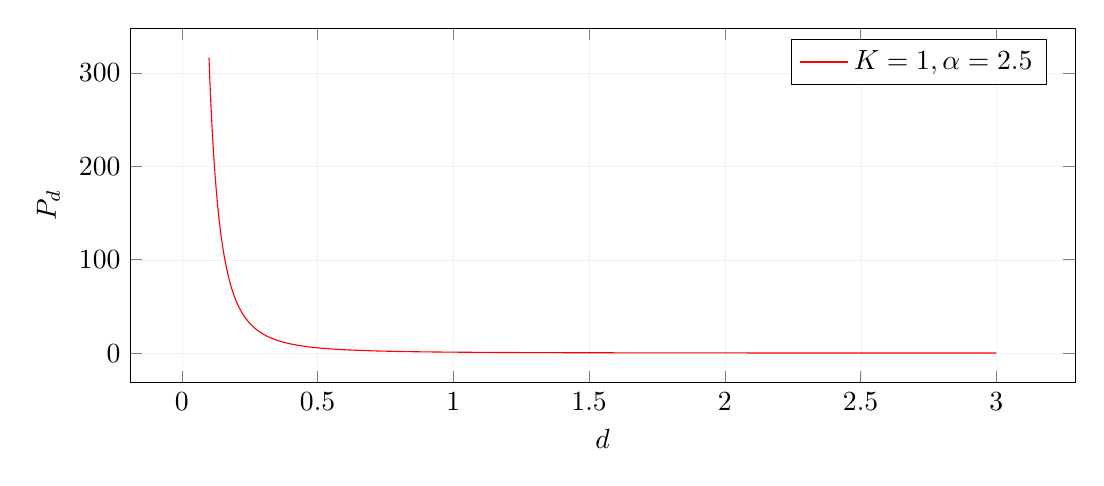
\begin{tikzpicture}[declare function={f(\x,\alpha,\k)=%
  (\k*pow(\x,-\alpha));}]
  %10*(\alpha-1)*pow(10*x,-\alpha);}]
     \begin{axis}[
      legend pos=north east,
      title = {},
      xlabel = {$d$},
      grid = both,
      grid style = {line width=.1pt, draw=gray!10},
      ylabel = {$P_d$},
      samples = 1000,
      width=12cm,height=4.5cm,
      enlargelimits=true,
      scale only axis=true]
    ]
      \addplot[red, no marks, domain=0.1:3, smooth]
      {f(x,2.5,1)};
      \addlegendentry{$K=1, \alpha = 2.5$}
    \end{axis}
  \end{tikzpicture}
  \caption{La rappresentazione non \`e del tutto corretta ($K$ dovrebbe fungere da costante di normalizzazione).}
\end{figure}

In questo tipo di grafi si ha spesso il fenomeno del \href{https://en.wikipedia.org/wiki/Preferential_attachment}{preferential attachment}, in cui quando un nuovo nodo si aggiunge al grafo \`e pi\`u probabile che si connetta ai nodi hub (quelli che hanno gi\`a tante connessioni). Ci possono essere quindi strutture molto diverse in termini di distribuzioni dei gradi.

\subsection{Connettività di un grafo}

Si definisce la matrice di adiacenza $A$:
\begin{equation}
\label{eqn:adjacency}
A_{ij} = \begin{cases}
    1, & \text{ se } \{i, j\} \in \mathcal{E} \\
    0, & \text{ altrimenti}
\end{cases}
\end{equation}
che fornisce una descrizione completa del grafo ed \`e utile per fare i calcoli. Si vede che che ogni riga somma al grado:
\begin{equation}
\sum_{j} A_{ij} = d_i
\end{equation}
e si ha poi che
\begin{equation}
A^2_{ij} = (AA)_{ij} = \sum_{k=1}^n A_{ik} A_{kj}
\end{equation}
in cui
\begin{equation}
A_{ik} A_{kj} \neq 0 \iff \{i,j\} \text{ sono collegati attraverso } k
\end{equation}
da cui si ha che $A^2_{ij}$ rappresenta il numero di \textbf{cammini di lunghezza} $2$ che connettono $i$ e $j$ e, in generale, $A^p_{ij}$ rappresenta il numero di cammini di lunghezza $p$ che connettono $i$ e $j$.

\begin{mybox}{green}{}
Tornando all'esempio \ref{exmp:grafoconn} si vede che
\begin{equation*}
    A = \begin{bmatrix}
    0 & 1 & 0 & 1 & 0 \\
    1 & 0 & 1 & 0 & 0 \\
    0 & 1 & 0 & 1 & 1 \\
    1 & 0 & 1 & 0 & 1 \\
    0 & 0 & 1 & 1 & 0
    \end{bmatrix}, \quad A^2 = \begin{bmatrix}
    2 & 0 & 2 & 0 & 1 \\
    0 & 2 & 0 & 2 & 1 \\
    2 & 0 & 3 & 1 & 1 \\
    0 & 2 & 1 & 3 & 1 \\
    1 & 1 & 1 & 1 & 2
    \end{bmatrix}, \quad A^3 = \begin{bmatrix}
    0 & 4 & 1 & 5 & 2 \\
    4 & 0 & 5 & 1 & 2 \\
    1 & 5 & 2 & 6 & 4 \\
    5 & 1 & 6 & 2 & 4 \\
    2 & 2 & 4 & 4 & 2
    \end{bmatrix}
\end{equation*}
\end{mybox}

Se si analizza $A^3_{ii}$ si può notare poi che questo rappresenta il numero dei \textit{triangoli} nel grafo aventi come vertice $i$ (in realt\`a sarebbe due volte questo numero dal momento che non \`e orientato)

%```dot
%Graph G{
%    x -- i -- y -- x
%}
%
%```

Quest'ultima propriet\`a pu\`o essere utile per studiare il \href{https://en.wikipedia.org/wiki/Clustering_coefficient}{\textbf{coefficiente di clustering}}:
\begin{equation}
\frac{\text{Tr} A^3}{\sum_{i \neq j} A^2_{ii}} = \frac{\sum{i=1} A^3_{ii}}{\sum_{i\neq j} A^2_{ij}} = \frac{6 \times \text{num. traingoli nel grafo}}{\text{num. triangoli potenziali}}
\end{equation}
in cui il numero di triangoli potenziali \`e il numero di coppie di nodi connesse da un cammino di lunghezza $2$.

Il coefficiente di clustering rappresenta la tendenza del grafo ad avere una struttura \textit{comunitaria}, ovvero una misura della presenza di cluster (\textbf{NB}: un triangolo \`e una comunit\`a di dimensione $3$).


\defn{\textit{Cammino:}} Un cammino di lunghezza $k$ tra due nodi $i_0, i_k$ in un grafo indiretto \`e una sequenza di nodi $c(i_0,i_k) = (i_0, i_1, \dots, i_k)$ tali che $\{i_{j-1}, i_j\} \in \mathcal{E}$. 

\defn{\textit{Grafo connesso:}} Un grafo si dice connesso quando, per ogni coppia di nodi $i,j$ esiste un cammino che li collega:
\begin{equation}
    \forall i,j \in \mathcal{N}: \exists \hspace{4pt} c(i,j)
\end{equation}

La connettivit\`a \`e quindi una propriet\`a (binaria) del grafo e ci chiediamo ora se sia possibile averne una misura quantitativa.
Esistono tanti modi, ovviamente: un modo per definire una misura del grado di connettivit\`a \`e attraverso la \textbf{distanza} $\delta_{ij}$, ovvero la \textit{lunghezza del cammino minimo} tra $i$ e $j$.\\
Tra le altre misure che ci possono interessare possiamo poi annoverare
\begin{itemize}
    \item Distanza \textit{media}: 
    \begin{equation}
        \bar{\delta} = \frac{1}{n(n-1)} \sum_{i \neq j} \delta_{ij}
    \end{equation}
    \item Distanza \textit{massima}: 
    \begin{equation}
        \delta_{max} = \max_{ij} \delta_{ij}
    \end{equation}
\end{itemize}
Queste misure sono importanti perch\`e rappresentano, o aiutano a quantificare, la velocit\`a di \textbf{diffusione dell'informazione} nel grafo (nel contesto di un SMA). 
In molti grafi (ad esempio quelli con distribuzioni \textit{power law}, ma non solo) si ha il cosidetto \href{https://en.wikipedia.org/wiki/Small-world_network}{small world effect}, ovvero in cui la distanza media $\bar{\delta}$ cresce lentamente (ad esempio come $\log n$) al crescere del numero $n$ di nodi del grafo.

Oltre alla velocit\`a di diffusione siamo anche interessati alla \textbf{robustezza} (della connettivit\`a rispetto alle disconnessioni) del grafo, che non pu\`o essere quantificata nei termini precedentemente introdotti.\\
Definiamo quindi due quantit\`a:
\begin{enumerate}
    \item La \textit{node connectivity} $\mathcal{V}_n$, ovvero il minimo numero di nodi che si devono rimuovere per rendere il grafo disconnesso.
    \item La \textit{edge connectivity} $\mathcal{V}_e$, ovvero il minimo numero di archi si devono rimuovere per rendere il grafo disconnesso.

\end{enumerate}
\begin{mybox}{green}{}
\begin{minipage}{0.5\textwidth}
\begin{tikzpicture}[-, >=stealth', auto, semithick, node distance=3cm]
\tikzstyle{every state}=[fill=white,draw=black,thick,text=black,scale=1]
    \node[shape=circle,draw=black] (A) at (0,0) {A};
    \node[shape=circle,draw=black] (B) at (1,1) {B};
    \node[shape=circle,draw=black] (C) at (1,-1) {C};
    \node[shape=circle,draw=black] (D) at (2,0) {D};
    \node[shape=circle,draw=black] (E) at (3,0) {E};
    \node[shape=circle,draw=black] (F) at (4,1) {F};
    \node[shape=circle,draw=black] (G) at (5,0) {G};

    \path (A) edge node[left] {} (B);
    \path (A) edge node[left] {} (C);
    \path (B) edge node[left] {} (C);
    \path (B) edge node[left] {} (D);
    \path (C) edge node[below] {} (D);
    \path (D) edge node[below] {} (E);
    \path (E) edge node[left] {} (F);
    \path (E) edge node[right] {} (G);
    \path (F) edge node[left] {} (G);
\label{fig:grafo2}
\end{tikzpicture}
\end{minipage}
\begin{minipage}{0.5\textwidth}
In una struttura come questa si ha, ad esempio, che $\mathcal{C}_n = \mathcal{C}_e = 1$ dal momento che basta togliere, rispettivamente, il nodo $D$ (o il nodo $E$) oppure l'arco tra i due per rendere il grafo disconnesso.
\end{minipage}
\end{mybox}

\subsection{Laplaciano di un grafo}

\`E uno strumento utile per studiare le propriet\`a di un grafo.
\defn{\textit{Matrice diagonale dei gradi:}} Dato un grafo $\mathcal{G} = (\mathcal{N}, \mathcal{E})$, indiretto non orientato, con $n=|\mathcal{N}|$, definiamo la \textbf{matrice diagonale dei gradi}:
\begin{equation}
    D \coloneqq diag\{d_1, d_2, \dots, d_n\}
\end{equation}
\defn{\textit{Laplaciano:}} Il \textbf{laplaciano} $\lap$ di un grafo (o matrice laplaciana) \`e definito come 
\begin{equation}
    \lap \coloneqq D - A
\end{equation}

dove $A$ \`e la matrice di adiacenza (definita in \ref{eqn:adjacency}).
\begin{mybox}{green}{\exmp{\textit{Calcolo del laplaciano di un grafo}}}
\label{exmp:lapla}
\begin{minipage}{0.5\textwidth}
\begin{center}
\begin{tikzpicture}[-, >=stealth', auto, semithick, node distance=3cm]
\tikzstyle{every state}=[fill=white,draw=black,thick,text=black,scale=1]
    \node[shape=circle,draw=black] (A) at (0,0) {$x_1$};
    \node[shape=circle,draw=black] (B) at (2,0) {$x_2$};
    \node[shape=circle,draw=black] (C) at (3,1) {$x_3$};
    \node[shape=circle,draw=black] (D) at (4,0) {$x_4$};

    \path (A) edge node[right] {} (B);
    \path (B) edge node[left] {} (C);
    \path (B) edge node[right] {} (D);
    \path (C) edge node[left] {} (D);
\end{tikzpicture} \end{center}
Considerando questo grafo si vede che
\begin{equation*}
D = \begin{bmatrix}
1 & 0 & 0 & 0 \\
0 & 3 & 0 & 0 \\
0 & 0 & 2 & 0 \\
0 & 0 & 0 & 2 \\
\end{bmatrix}
\text{ e }
A = \begin{bmatrix}
0 & 1 & 0 & 0 \\
1 & 0 & 1 & 1 \\
0 & 1 & 0 & 1 \\
0 & 1 & 1 & 0 \\
\end{bmatrix}
\end{equation*}
\end{minipage}
\begin{minipage}{0.5\textwidth}
da cui si ha (notando che la matrice di adiacenza \`e una matrice \textbf{simmetrica per un grafo indiretto}) il laplaciano
\begin{equation*}
\lap = D - A = \begin{bmatrix}
-1 & -1 & 0 & 0 \\
-1 & 3 & -1 & -1 \\
0 & -1 & 2 & -1 \\
0 & -1 & -1 & 2 \\
\end{bmatrix}
\end{equation*}
\end{minipage}
\end{mybox}

In generale si ha che, definendo $\mathcal{N}_i$ l'insieme dei vicini del nodo $i$
\begin{equation}
\lap_{i,j} \coloneqq \begin{cases}
d_i, & j=i \\
-1, & j \in \mathcal{N}_i\\
0, & \text{altrimenti }
\end{cases}
\end{equation}

il laplaciano contiene quindi \textit{tutte} le propriet\`a del grafo, cos\`i come la matrice di adiacenza, e il loro uso (del laplaciano o della matrice di adiacenza) dipende dall'applicazione. Elenchiamo alcune delle
\textbf{propriet\`a} del Laplaciano:
\begin{enumerate}
\item Ogni riga somma a $0$.
        \[ \sum_{j} \lap_{ij} = 0 \]
\item \`E una matrice simmetrica (quando il grafo \`e indiretto), ovvero $\lap = \lap^\intercal$.
\item Anche le colonne sommano a $0$ (per la simmetria, quindi solo nei grafi indiretti).
        \[ \sum_{i} \lap_{ij} = 0 \]
\item \`E una matrice diagonale dominante.
        \[ \lap_{ii} = \sum_{i \neq j} |L_{ij}| \]
\item \`E una matrice semidefinita positiva.
        \[ x^\intercal \lap x \geq 0, \quad \forall x \in \mathbb{R}^n \]
\item Detta $M$ la matrice di incidenza del grafo vale $\lap = M^\intercal M$ (vedi sez. \ref{sec:lapinc}).
\end{enumerate}
Dimostriamo la 5.:
\begin{tcolorbox}[enhanced,breakable,frame hidden]
\textbf{Dim:} Si vuole mostrare quindi che $x^\intercal \lap x \geq 0, \forall x \in \mathbb{R}^n$.
Si ha che
\begin{align*}
x^\intercal \lap x &= \sum_{i=1}^n \sum_{j=1}^n \lap_{i,j} x_i x_j = \\
&= \sum_{i=1}^n \Big ( L_{i,i} x_i^2 + \sum_{j\neq1} L_{i,j} x_i x_j \Big ) = \\ 
&= \sum_{i=1}^n \Big (d_i x_i^2 + \sum_{j \in \mathcal{N}_i} -x_i x_j \Big ) = \\
&= \sum_{i=1}^n \Big ( \sum_{j \in \mathcal{N}_i} x_i^2 - x_i x_j \Big )
\end{align*}
si ha poi che la somma per tutti i nodi per ogni vicino pu\`o essere pensata circa come la somma su tutti gli archi
\begin{equation*}
\sum_{i=1}^n \sum_{j \in \mathcal{N}_i} \approx \sum_{\{i,j\} \in \mathcal{E}}
\end{equation*}
in particolare, dato che queste sommatorie considerano tutti gli archi due volte (una volta come $\{i,j\}$ e una volta come $\{j,i\}$) si ha
\begin{align*}
x^\intercal \lap x &= \sum_{i=1}^n \sum_{j \in \mathcal{N}_i} x_i^2 - x_i x_j \\
&= \sum_{\{i,j\} \in \mathcal{E}} (x_i^2 - x_i x_j + x_j^2 - x_i x_j) = \\ 
&= \sum_{\{i,j\} \in \mathcal{E}} (x_i - x_j)^2 \geq 0, \qquad \forall x.
\end{align*}
\[
\square
\]
\end{tcolorbox}
\begin{mybox}{green}{}
Seguendo l'esempio \ref{exmp:lapla} avremo quindi, detto $x$ il vettore complessivo degli stati $x = [x_1, x_2, x_3, x_4]^\intercal$:
\begin{align*}
x^\intercal \lap x &= [x_1, x_2, x_3, x_4] \begin{bmatrix}
-1 & -1 & 0 & 0 \\
-1 & 3 & -1 & -1 \\
0 & -1 & 2 & -1 \\
0 & -1 & -1 & 2 \\
\end{bmatrix} \begin{bmatrix} x_1 \\ x_2 \\ x_3 \\ x_4 \end{bmatrix} \\
&= (x_1 - x_2)^2 + (x_2 - x_3)^2 + (x_3 - x_4)^2 + (x_2 - x_4)^2
\end{align*}
\end{mybox}

\subsubsection{Relazione tra Laplaciano e matrice d'incidenza}
\label{sec:lapinc}

Supponendo di assegnare un valore $x_i$ a ciascun nodo, allora $x^\intercal \lap x$ \textbf{misura il disaccordo} (nel senso della distanza totale) tra nodi vicini. 
Nell'esempio se $x_1$ e $x_2$ fossero nello stesso stato ($x_1 = x_2$) si avrebbe distanza nulla.

Per calcolare $x^\intercal \lap x$ si pu\`o costruire il vettore \textbf{vettore dei collegamenti} (seguendo l'esempio 1):
\begin{equation}
 \xi = 
\begin{bmatrix}
x_1 - x_2 \\
x_2 - x_3 \\
x_2 - x_4 \\
x_3 - x_4 
\end{bmatrix}
\end{equation}
e calcolarne il prodotto scalare (in norma 2):
\begin{equation}
    \| \xi \|^2_2 = \xi^\intercal \xi = x^\intercal \lap x
\end{equation}

Si ha inoltre che, in generale, il vettore $\xi$ puo essere ottenuto da $x$ tramite la \textbf{matrice di incidenza} del grafo, $M$:
\begin{equation}
\xi = M x
\end{equation}

\defn{\textit{Matrice di incidenza:}} La matrice d'incidenza $M$ \`e una matrice $|\mathcal{E}| \times |\mathcal{N}|$ in cui ogni riga corrisponde a un arco e ogni colonna corrisponde a un nodo. Se la riga $k$ di $M$ \`e associata all'arco $\{i, j\}$ allora
\begin{equation}
M_{kl} \coloneqq \begin{cases}
1, & \text{ per $l = i$ }\\
-1, & \text{ per $l = j$ }\\
0, & \text{ altrimenti }
\end{cases}
\end{equation}
\textbf{N.B:} Ogni riga \`e definita a meno di un segno perche il grafo \`e non orientato.
\begin{mybox}{green}{}
Seguendo ancora l'esempio \ref{exmp:lapla} si ha
\[
\xi = \underbrace{\begin{bmatrix}
1 & -1 & 0 & 0 \\
0 & 1 & -1 & 0 \\
0 & 1 & 0 & -1 \\
0 & 0 & 1 & -1 
\end{bmatrix}}_{M}
\underbrace{\begin{bmatrix}
x_1 \\
x_2 \\
x_3 \\
x_4
\end{bmatrix}}_{x} = \begin{bmatrix} x_1 - x_2 \\ x_2 - x_3 \\ x_2 - x_4 \\ x_3 - x_4 \end{bmatrix}
\]
\end{mybox}
Si vede infine che:
\begin{equation}
x^\intercal \lap x = \xi^\intercal \xi = (Mx)^\intercal(Mx) = x^\intercal M^\intercal M x
\end{equation}
da cui abbiamo l'ultima propriet\`a del laplaciano, cio\`e che
\begin{equation}
    \lap = M^\intercal M
\end{equation}

\subsubsection{Cenni alla Teoria Spettrale}
Poiche $\lap$ \`e una matrice $n\times n$ simmetrica si ha che tutti i suoi autovalori $\lambda_1, \lambda_2, \dots, \lambda_n$ sono reali.

A ciascun autovalore $\lambda_i$ \`e associato un autovettore $v_i$ con la propriet\`a
\begin{equation}
\lap v_i = \lambda_i v_i
\end{equation}
Una matrice simmetrica pu\`o sempre essere decomposta come
\begin{equation}
\lap = V \Lambda V^\intercal
\end{equation}
dove $\Lambda = diag\{\lambda_1, \dots, \lambda_n\}$ e $V = [v_1, \dots, v_n]$ \`e la matrice \textbf{ortogonale} degli autovettori (avente per colonne gli autovettori). Una conseguenza del fatto che $V$ sia una matrice ortogonale \`e che $V^{-1} = V^\intercal$.\\
Quindi una matrice simmetrica \`e \textit{completamente caratterizzata} dai suoi autovalori e dai suoi autovettori ed \textbf{il grafo quindi pu\`o essere codificato attraverso gli autovalori e gli autovettori del laplaciano}. Da qui si \`e sviluppata una teoria che ha come obiettivo lo studio degli autovalori e degli autovettori del laplaciano che prende il nome di \href{https://en.wikipedia.org/wiki/Spectral_graph_theory}{Teoria Spettrale dei grafi}.

Essendo $\{\lambda_1, \dots, \lambda_n\} \in \mathbb{R}$ possiamo ordinarli in modo crescente, supponendo, senza perdita di generalit\`a, di avere questa struttura:
\begin{equation}
0 \leq \lambda_1 \leq \lambda_2 \leq \dots \leq \lambda_n
\end{equation}
dal momento che, essendo $\lap$ semidefinita positiva, si ha che $\lambda_i \geq 0, \forall i \in \{1, \dots, n\}$.\\
In realt\`a \textbf{per ogni grafo vale}:
\begin{equation}
\lambda_1 = 0 \text{ con autovettore associato } v_1 = \frac{1}{\sqrt{n}} \begin{bmatrix}
1 \\
1 \\
\vdots \\
1
\end{bmatrix} = \frac{1}{\sqrt{n}} \underline{1} \hspace{5pt}\text{ per costruzione.}
\end{equation}
Infatti \`e facile vedere che $\lap \underline{1} = 0$ quindi non ci da particolare informazioni sul grafo dal momento che \`e \textbf{vero per tutti}, infatti:
\begin{equation}
\lap \underline{1} = \begin{bmatrix}
\lap_{11} + \lap_{12} + \dots \lap_{1n} \\
\vdots \\
\lap_{n1} + \lap_{n2} + \dots \lap_{nn}
\end{bmatrix} = \begin{bmatrix}
0 \\
\vdots \\
0
\end{bmatrix}
\end{equation}

perch\`e tutte le righe di $\lap$ sommano a 0. Si ha poi quindi che
\begin{equation}
\lap \alpha \underline{1} = \alpha \lap \underline{1} = 0, \quad \forall \alpha \in \mathbb{R}
\end{equation}
Un altro modo per vederlo \`e analizzando la forma quadratica
\begin{equation}
x^\intercal \lap x = \sum_{\{i,j\} \in \mathcal{E}} (x_i - x_j)^2
\end{equation}
prendendo $x = \alpha \underline{1} = \begin{bmatrix} \alpha \\ \vdots \\ \alpha \end{bmatrix}$ si ha che
\begin{equation}
x^\intercal \lap x = \sum_{\{i,j\} \in \mathcal{E}} (\alpha - \alpha)^2 = 0
\end{equation}
in cui quindi si ha \textbf{disaccordo nullo}.\\
Si pu\`o dimostrare poi che per qualsiasi grafo non orientato vale che il massimo degli autovalori 
\begin{equation}
    \lambda_n \leq 2 d_{max}
\end{equation} dove $d_{max} = \max_{i} d_i$ (ovvero il grado massimo tra tutti i nodi). 
Vale quindi in definitiva che:
\begin{equation}
0 = \lambda_1 \leq \lambda_2 \leq \dots \leq \lambda_n \leq 2 d_{max}
\end{equation}

\subsection{Connettivit\`a algebrica}

Concentraimoci adesso su un oggetto fondamentale: il secondo autovalore $\lambda_2$. Questo prende il nome di \textbf{connettivit\`a algebrica del grafo} (anche detto \textit{autovalore di Fiedler}) e ci da informazione appunto sulla connettivit\`a del grafo. 

Per prima cosa vale che, per un grafo indiretto:
\begin{equation}
\lambda_2 > 0 \iff \text{ il grafo \`e connesso }
\end{equation}
Oltre a fornire un'informazione binaria (connesso-non connesso) ci da una \textbf{misura quantitativa} della connettivit\`a di un grafo, in quanto pi\`u il grafo \`e connesso pi\`u grande risulta $\lambda_2$. Questo autovalore tiene conto \textit{sia} della velocit\`a con cui si diffonde l'informazione \textit{sia} della robustezza rispetto a disconnessioni di nodi/archi.\\
Vale infatti che 
\begin{equation}
\lambda_2 \leq \mathcal{V}_n \leq \mathcal{V}_e
\end{equation}
dove $\mathcal{V}_n, \mathcal{V}_e$ sono, rispettivamente, la \textit{node connectivity} e la \textit{edge connectivity}.

Per grafi con struttura "semplice" $\lambda_2$ si calcola analiticamente, ad esempio nel \textit{grafo completo} si ha $\lambda_2 = n$ (molto connesso), nel \textcolor{red}{\textit{grafo bipartito}} si ha $\lambda_2 = n/2$ mentre nel \textcolor{green}{\textit{grafo a stella}} si ha $\lambda_2 = 1$ (molto poco connesso).\\
In un \textcolor{blue}{\textit{ciclo}} si ha, con conti un po piu lunghi, $\lambda_2 = 2[1 - \cos (2\pi/n)]$, infatti quando $n$ cresce il grafo perde connettivit\`a (il $\cos \to 1$ e $\lambda_2 \to 0$). Per un \textcolor{orange}{\textit{cammino}} si ha $\lambda_2 = 2[1 - cos(\pi/n)]$.

\begin{center}
    \begin{tikzpicture}[-, >=stealth', auto, semithick, node distance=3cm]
    \tikzstyle{every state}=[fill=white,draw=black,thick,text=black,scale=1]
    \node[shape=circle,draw=black] (A) at (0,0) {};
    \node[shape=circle,draw=black] (B) at (0,1) {};
    \node[shape=circle,draw=black] (C) at (1,0) {};
    \node[shape=circle,draw=black] (D) at (1,1) {};
    
    \node[shape=circle,draw=red] (1) at (2,1) {};
    \node[shape=circle,draw=red] (2) at (3,1) {};
    \node[shape=circle,draw=red] (3) at (4,1) {};
    \node[shape=circle,draw=red] (4) at (2,0) {};
    \node[shape=circle,draw=red] (5) at (3,0) {};
    \node[shape=circle,draw=red] (6) at (4,0) {};
    
    \node[shape=circle,draw=green] (x) at (6,0.5) {};
    \node[shape=circle,draw=green] (y) at (6,1) {};
    \node[shape=circle,draw=green] (z) at (7,0.5) {};
    \node[shape=circle,draw=green] (w) at (6,0) {};
    \node[shape=circle,draw=green] (q) at (5,0.5) {};
    
    \node[shape=circle,draw=blue] (e) at (8,0) {};
    \node[shape=circle,draw=blue] (f) at (8,1) {};
    \node[shape=circle,draw=blue] (g) at (9,0) {};
    \node[shape=circle,draw=blue] (h) at (9,1) {};
    
    \node[shape=circle,draw=orange] (i) at (10,0.5) {};
    \node[shape=circle,draw=orange] (l) at (11,0.5) {};
    \node[shape=circle,draw=orange] (m) at (12,0.5) {};
    \node[shape=circle,draw=orange] (n) at (13,0.5) {};

    \path (A) edge node {} (B);
    \path (A) edge node {} (C);
    \path (A) edge node {} (D);
    \path (B) edge node {} (C);
    \path (B) edge node {} (D);
    \path (C) edge node {} (D);
    
    \path (1) edge[draw=red] node {} (4);
    \path (1) edge[draw=red] node {} (5);
    \path (1) edge[draw=red] node {} (6);
    \path (2) edge[draw=red] node {} (4);
    \path (2) edge[draw=red] node {} (5);
    \path (2) edge[draw=red] node {} (6);
    \path (3) edge[draw=red] node {} (4);
    \path (3) edge[draw=red] node {} (5);
    \path (3) edge[draw=red] node {} (6);
    
    \path (x) edge[draw=green] node {} (y);
    \path (x) edge[draw=green] node {} (z);
    \path (x) edge[draw=green] node {} (w);
    \path (x) edge[draw=green] node {} (q);
    
    \path (e) edge[draw=blue] node {} (f);
    \path (f) edge[draw=blue] node {} (h);
    \path (g) edge[draw=blue] node {} (h);
    \path (g) edge[draw=blue] node {} (e);
    
    \path (i) edge[draw=orange] node {} (l);
    \path (m) edge[draw=orange] node {} (l);
    \path (m) edge[draw=orange] node {} (n);
\end{tikzpicture}
\end{center}

Per grafi con struttura pi\`u complicata si vanno ad utilizzare tecniche di analisi numerica per ricavare il valore di $\lambda_2$.

Vediamo ora una propriet\`a della connettivit\`a algebrica:

\begin{equation}
\begin{cases}
\text{Grafo connesso} \iff \lambda_2 >0 \iff \text{ l'autovalore in 0 ($\lambda_1)$ ha molteplicit\`a 1}\\
\text{Grafo non connesso }\iff \lambda_2 = 0
\end{cases}
\end{equation}

\begin{tcolorbox}[enhanced, breakable, frame hidden]
\textbf{Dim}: Consideriamo la forma quadratica
\[
x^\intercal \lap x = \sum_{\{i,j\}} (x_i - x_j)^2
\]
abbiamo visto che $x^\intercal \lap x = 0$ quando $x = \alpha \underline{1}$. L'autovalore in 0 ha molteplicit\`a 1 se e solo se non ci sono vettori diversi da $\alpha \underline{1}$ tali che $x^\intercal \lap x = 0$ (o equivalentemente $Lx = 0$), ovvero se e solo se il mio laplaciano si annulla solo in una direzione (se ci fossero altri vettori avrei altre direzioni in cui si annulla il laplaciano).\\
Nel caso di \textbf{grafo connesso} quindi, considerando quella forma quadratica, si ha che
\[
x^\intercal \lap x = 0 \iff x_i - x_j = 0, \qquad \forall \{i,j\} \in \mathcal{E}
\]
ovvero che tutti i nodi assumano lo stesso valore:
\[
x^\intercal \lap x = 0 \iff x_i = x_j
\]
questo per ogni coppia di nodi, non necessariamente collegati da un arco.
Per un grafo connesso si ha quindi che:
\[
x^\intercal \lap x = 0 \iff \exists \alpha: x_i = \alpha, \forall i
\]
ovvero in cui l'autovalore in 0 ha molteplicit\`a 1, che implica $\lambda_2 > 0$.

Nel caso di grafo \textbf{non connesso} invece $x^\intercal \lap x$ si annulla anche quando non tutti i valori associati ai nodi sono coincidenti, questo implica che l'autovalore in 0 ha molteplicit\`a $>1$ e quindi che $\lambda_2 = 0$.
\[
\square
\]
\end{tcolorbox}
\begin{mybox}{green}{}
\begin{minipage}{0.3\textwidth}
\begin{tikzpicture}[-, >=stealth', auto, semithick, node distance=3cm]
\tikzstyle{every state}=[fill=white,draw=black,thick,text=black,scale=1]
    \node[shape=circle,draw=black] (A) at (0,0) {$a$};
    \node[shape=circle,draw=black] (B) at (1.5,0) {$b$};
    \node[shape=circle,draw=black] (C) at (2,1) {$c$};
    \node[shape=circle,draw=black] (D) at (3,0) {$d$};

    \path (A) edge node[right] {} (B);
    \path (C) edge node[left] {} (D);
\end{tikzpicture}
\end{minipage}
\begin{minipage}{0.7\textwidth}
In questo semplice caso si ha 
\begin{equation*}
    x^\intercal \lap x = (a - b)^2 + (c- d)^2 = 0 \iff a=b \land c=d
\end{equation*} 
e quindi non implica che tutti i valori debbano essere necessariamente uguali tra loro.
\end{minipage} \hspace{4pt}
\end{mybox}

In generale vale che il numero $n_0$ di autovalori in 0 (autovalori nulli) di $\lap$ \`e pari al numero di \textbf{componenti connesse} del grafo.
Nell'esempio appena fatto si avrebbe $\lambda_1 = \lambda_2 = 0$ e $\lambda_3 > 0$.

In generale se si hanno $N$ componenti connesse si pu\`o definire un laplaciano $\lap_k$ per ogni componente connessa e (\textit{eventualmente riordinando i nodi}) si ha che il laplaciano complessivo sar\`a una matrice diagonale a blocchi:
\begin{equation}
\lap = \begin{bmatrix}
\lap_1 & 0 & \dots & 0 \\
0 & \lap_2 & \dots & 0 \\
\vdots & \vdots & \ddots & \vdots \\
0 & 0 & \dots & \lap_N
\end{bmatrix}
\end{equation}

da cui si vede che gli autovalori di $\lap$ sono gli autovalori di $\lap_1$, gli autovalori di $\lap_2, \dots$, autovalori di $\lap_N$ in cui si ha 1 autovalore in 0 per ogni componente connessa $k$ (quindi si hanno $N$ autovalori in zero). Questo vuol dire che:
\begin{equation}
\text{rank }\lap = n - N
\end{equation}
dove $n = |\mathcal{N}|$ \`e il numero di nodi e $N$ il numero di componenti connesse.

Le considerazioni fatte fin ora valgono anche per \textbf{grafi pesati non orientati}: La definizione del laplaciano cambia solo minimamente.
\begin{mybox}[breakable]{green}{}
Consideriamo ad esempio un semplice grafo pesato di questo tipo
\begin{center}
\begin{tikzpicture}[-, >=stealth', auto, semithick, node distance=3cm]
\tikzstyle{every state}=[fill=white,draw=black,thick,text=black,scale=1]
    \node[shape=circle,draw=black] (1) at (0,0) {$1$};
    \node[shape=circle,draw=black] (2) at (2,0) {$2$};
    \node[shape=circle,draw=black] (3) at (3,1) {$3$};
    \node[shape=circle,draw=black] (4) at (4,0) {$4$};

    \path (1) edge node[midway] {$a_{12}$} (2);
    \path (2) edge node[midway] {$a_{23}$} (3);
    \path (2) edge node[midway] {$a_{24}$} (4);
    \path (3) edge node[midway] {$a_{34}$} (4);
\end{tikzpicture}
\end{center}
Si ha una matrice di adiacenza
\begin{equation*}
A = \begin{bmatrix}
0 & a_{12} & 0 & 0 \\
a_{12} & 0 & a_{23} & a_{24} \\
0 & a_{23} & 0 & a_{34} \\
0 & a_{24} & a_{34} & 0
\end{bmatrix}
\end{equation*}
e quindi un Laplaciano
\begin{equation*}
\lap = \begin{bmatrix}
a_{12} & -a_{12} & 0 & 0 \\
-a_{12} & a_{12} + a_{23} + a_{24} & -a_{23} & -a_{24} \\
0 & -a_{23} & a_{23} + a_{34} & -a_{34} \\
0 & -a_{24} & -a_{34} & a_{24} + a_{34}
\end{bmatrix}
\end{equation*}
\end{mybox}
In generale
\begin{equation}
\lap_{ij} = \begin{cases}
-a_{ij}, & j \in \mathcal{N}_i \\
\sum_{k}a_{ik}, & j=i, k \in \mathcal{N}_i \\
0, & \text{altrimenti}
\end{cases}
\end{equation}

e continuano a valore le stesse propriet\`a, semplicemente entrano in gioco i pesi:
\begin{enumerate}
\item \`E simmetrico (nel caso indiretto).
\item Righe e colonne sommano a 0.
\item \`E semidefinito positivo.
\item $x^\intercal \lap x = \sum_{\{i,j\} \in \mathcal{E}} a_{ij} (x_i - x_j)^2$.
\item $\lambda_1 = 0, \lambda_2 > 0 \iff$ il grafo \`e connesso.
\end{enumerate}

\subsection{Partizionamento di un grafo e clustering spettrale}

Supponiamo di avere un grafo $\mathcal{G}$, vogliamo dividere il grafo in 2 parti: $C_1, C_2$ tali che $C_1 \cup \mathcal{C}_2 = \mathcal{N}$, $C_1 \cup C_2 = \emptyset$ e tali che $C_1 \neq \emptyset, C_2 \neq \emptyset$. Si vuole:
\begin{enumerate}
\item Avere pochi collegamenti tra nodi appartenenti a gruppi diversi.
\item Avere tanti collegamenti tra nodi appartenenti allo stesso gruppo.
\end{enumerate}

\textbf{Idea semplice}: Si scelgono $C_1, C_2$ in modo da minimizzare il numero di collegamenti $\{i, j\}$ con $i\in C_1$ e $j \in C_2$. Questo \textit{equivale a trovare il taglio del grafo che attraversa il minor numero di archi}, ovvero risolvere il problema del \href{https://en.wikipedia.org/wiki/Minimum_cut}{MinCut}. Matematicamente quindi, data una partizione $\{C_1, C_2\}$ si pu\`o assegnare un valore $x_i$ in questo modo:
\begin{equation}
x_i = \begin{cases}
1, & i \in C_1 \\
-1, & i \in C_2
\end{cases}
\end{equation}
ovvero \textit{assegnare un'etichetta} $\{+1, -1\}$ ad ogni nodo. 
Consideriamo ora il costo $J(x)$:
\begin{equation}
J(x) = \frac{1}{4} x^\intercal \lap x = \frac{1}{4} \sum_{i,j} (x_i - x_j)^2
\end{equation}
da cui si ha che
\begin{equation}
(x_i - x_j)^2 = \begin{cases}
0, \quad \text{se } \{i,j\} \in C_1 \lor \{i,j\} \in C_2 \\
4, \quad \text{se } i \in C_1, j\in C_2 \lor i \in C_2, j \in C_1
\end{cases}
\end{equation}
ovvero che il costo $J$ rappresenta il \textit{numero di collegamenti tra nodi appartenenti a cluster diversi}, esprime cio\`e il \textbf{disaccordo totale}. Il problema del MinCut pu\`o essere quindi espresso in termini del Laplaciano come:
\begin{align*}
\min_{x \in \{-1, 1\}^n} \quad &\frac{1}{4} x^\intercal \lap x \\
\text{s.t } \quad &x \neq \underline{1} \land x \neq -\underline{1}
\end{align*}
dove il vincolo ci dice che i cluster \textit{non devono essere vuoti}. Questo \`e un problema di ottimizzazione \textit{combinatorio} perch\`e le variabili $x_i$ sono discrete (in questo caso binarie), tuttavia pu\`o essere risolto in tempo polinomiale, attraverso l'algoritmo di \href{https://en.wikipedia.org/wiki/Stoer-Wagner_algorithm}{Stoer-Wagner}. In realt\`a questo algoritmo si usa principalmente per trovare la edge connectivity, non si usa nella pratica per trovare il MinCut dal momento che, per certi grafi, ha la tendenza a fare partizioni molto \textbf{sbilanciate}, in cui si ha che $C_1$ e $C_2$ possono avere dimensione molto diversa.

\textbf{Idea 2}: Vogliamo quindi imporre un certo bilanciamento. Questo pu\`o essere fatto ad esempio imponendo $|C_1| = |C_2|$, supponendo $n$ pari, ovvero aggiungendo il vincolo:
\begin{equation}
\sum_{i=1}^n x_i = x^\intercal \underline{1} = 0
\end{equation}
Potremmo quindi pensare di risolver questo nuovo problema, in cui adesso \`e sufficiente solo questo vincolo:
\begin{align*}
\min_{x \in \{-1, 1\}^n} \quad &\frac{1}{4} x^\intercal \lap x \\
\text{s.t } \quad &x^\intercal \underline{1} = 0
\end{align*}
Questo per\`o porta a due \textit{difficoltà}: fa esplodere la complessità computazione da polinomiale a \textit{$NP$-hard} e, in secondo luogo, scegliere a priori la dimensione dei cluster non \`e consigliabile.

\textbf{Idea 3}: La soluzione pu\`o essere quella di rilassare il vincolo di integrit\`a, svincolando da $x \in \{-1, 1\}^n$ a $x \in \mathbb{R}^n$ ma mantenendo il passaggio per $\{-1, 1\}^n$, ovvero preservando la norma imponendo $\| x \|^2 = x^\intercal x = n$. 
Per partizionare il grafo si risolve quindi infine il problema:
\begin{align*}
\min_{x \in \mathbb{R}^n} \quad &\frac{1}{4} x^\intercal \lap x \\
\text{s.t } \quad &x^\intercal x = n \\
&x^\intercal \underline{1} = 0
\end{align*}
Il vettore ottenuto sar\`a quindi formato da componenti continue: dopo aver risolto il problema si assegna quindi, ad esempio:
\begin{equation}
i \in C_1 \text{ se } x_i > 0, \qquad i \in C_2 \text{ se } x_i < 0 
\end{equation}
come regola di decisione per assegnare il nodo $i$-esimo ad un cluster. La soglia non deve essere necessariamente a 0 ma pu\`o essere scelta secondo un qualche criterio (ad esempio seguendo tecniche di clustering). 

Analizziamo la struttura della soluzione:
Dato il Laplaciano $\lap$ considero la connettivit\`a algebrica $\lambda_2$ e il corrispondente autoversore $v_2$:
\begin{equation}
\lap v_2 = \lambda_2 v_2, \qquad v_2^\intercal v_2 = 1
\end{equation}
allora la \textbf{soluzione $\hat{x}$ del problema formulato} \`e data da:
\begin{equation}
\hat{x} = \frac{v_2}{\sqrt{n}}
\end{equation}
ed il costo minimo $\hat{J}$ vale:
\begin{equation}
\hat{J} = \frac{\lambda_2}{n}
\end{equation}

In generale, se si vuole suddividere il grafo in $K$ gruppi, si pu\`o procedere in due modi:
\begin{enumerate}
    \item Iterativamente: prima si divide in 2 gruppi, poi in 4, e cos\`i via. Per dividere un grafo in due sottografi si deve quindi
    \begin{itemize}
        \item Calcolare $\lap$
        \item Calcolare $v_2$
        \item Esaminare, per ogni nodo $i$, la $i$-esima componente del vettore $v_2$ e decidere
        \begin{equation}
            \begin{cases}
                i \in C_1 &\text{se } v_{2_i} > 0 \\
                i \in C_2 &\text{se } v_{2_i} < 0
            \end{cases}
        \end{equation}
    \end{itemize}
    \item Utilizzando \textit{anche} gli autovettori successivi di $\lap: v_3, \dots, v_K$. Partendo dalla decomposizione autovalore-autovettore:
    \[
    \lap = V \Lambda V^\intercal
    \]
    si va a costruire, dalla matrice $n\times n$ ortonormale degli autovettori $V$, per ogni nodo $i$, un vettore
    \[
    x_i = \begin{bmatrix}
    v_{2_i} \\
    v_{3_i} \\
    \vdots \\
    v_{K_i}
    \end{bmatrix}
    \]
    e si partiziona il grafo usando una qualche tecnica di clustering (ad esempio $k$-means) per clusterizzare i vettori $x_1, \dots, x_N$.
\end{enumerate}

Questo ci mostra come anche \textit{gli autovalori del Laplaciano ci diano informazioni importanti sulla struttura topologica} del grafo.

\subsubsection{Cenni al clustering spettrale}

Queste idee si applicano anche al problema del clustering: 
Dati $z_1, z_2, \dots, z_N$ punti in $\mathbb{R}^n$, allora sulla base della distanza (o rispetto ad una funzione di similarit\`a) si vuole dividerli in $K$ gruppi (cluster) $C_1, \dots, C_K$ separati (tali cio\`e che $C_i \cap C_j = \emptyset$) in modo che:
\begin{itemize}
\item Punti appartenenti allo stesso cluster siano simili tra loro.
\item Punti appartenenti a cluster diversi siano dissimili.
\end{itemize}

La somiglianza pu\`o essere misurata ad esempio attraverso la norma euclidea con $\| z_i - z_j \|$.

Un algoritmo tipico di clustering \`e il \href{https://en.wikipedia.org/wiki/K-means_clustering}{\textit{k-means}}, che si basa sull'idea di individuare $K$ centroidi ed assegnare i punti al centroide pi\`u vicino. Questo algoritmo funziona quando i cluster sono effettivamente distribuiti intorno ai centroidi (come in figura \ref{fig:clusconv}), altrimenti no.\\
Tipicamente il $k$-means non funziona quando si devono separare cluster non convessi, come in figura \ref{fig:nonconv} (in cui si ha una struttura di due cluster concentrici, che l'algoritmo non \`e in grado di individuare):
\begin{figure}[!htbp]
  \centering
  \begin{minipage}[b]{0.4\textwidth}
    \includegraphics[scale=0.6]{img/kmeans2.png}
    \caption{Cluster separati.}
    \label{fig:clusconv}
  \end{minipage}
  \hfill
  \begin{minipage}[b]{0.4\textwidth}
    \includegraphics[width=\textwidth]{img/plot_kmeans-1.png}
    \caption{Cluster non convessi.}
    \label{fig:nonconv}
  \end{minipage}
\end{figure}


Il clustering spettrale invece risulta efficace:

\begin{enumerate}
\item Dati i punti $z_1, \dots, z_N$ costruisco un grafo $\mathcal{G} = (\mathcal{N}, \mathcal{E})$ sulla base della loro similarit\`a.
\item Si determina il Laplaciano $\lap$ del grafo $\mathcal{G}$.
\item Si determina i primi $K$ autovettori $v_1, v_2, \dots, v_K$ (il primo non servirebbe dal momento che \`e sempre in zero).
\item Per ogni dato $z_i$ a cui \`e associato il nodo $i$ si costruisce il vettore delle componenti
    \begin{equation}
    x_i = \begin{bmatrix}
    v_{2_i} \\
    v_{3_i} \\
    \vdots \\
    v_{K_i}
    \end{bmatrix}
    \end{equation}
\item Si applica un algoritmo di clustering (es. $k$-means) ai punti $x_1, \dots, x_N$.
\end{enumerate}
Per costruire $\mathcal{G}$ esistono diverse strategie:
\begin{enumerate}
\item Metodo $\epsilon$-neighborhood: $\{i,j\} \in \mathcal{E} \iff \| x_i - x_j \| \leq \epsilon$ in cui $\epsilon$ \`e un iperparametro. In questo modo si costruisce un grafo geometrico non pesato.
\item Metodo $h$-nearest-neeighbors: per ogni punto $z_i$ si cercano gli $h$ punti pi\`u vicini: $\{i,j \} \iff j$ \`e uno dei primi $h$ vicini di $i$ o $i$ \`e uno dei primi $h$ vicini di $j$. In questo modo si costruisce simmetricamente un grafo non orientato e non pesato.
\item Costruire un grafo completamente connesso e pesato: all'arco $\{i,j\}$ si assegna un peso $a_{ij}$ che dipende dalla distanza tra $z_i$ e $z_j$, ad esempio prendendo 
   \begin{equation}
   a_{ij} = \exp \Big \{ {-\frac{\| z_i - z_j \|^2}{2\sigma^2}} \Big \}
   \end{equation}
   in cui scegliere $\sigma$ \`e meno critico che scegliere $\epsilon$: quest'ultimo infatti ci porta a una connettivit\`a binaria: connesso o non connesso, con $\sigma$ riusciamo a mitigare questo fenomeno andando ad utilizzare un parametro continuo per indicare la forza della connessione. Questo pu\`o essere quindi visto come un rilassamento del primo metodo.
\end{enumerate}

In alternativa esistono tecniche come \href{https://it.wikipedia.org/wiki/Dbscan}{\textit{DBSCAN}} che cercano di costruire un grafo gi\`a diviso in componenti separate tra loro anche se, come nel caso di DBSCAN, sono generalizzazioni del primo approccio e quindi si portano dietro la criticit\`a della scelta di $\epsilon$. In grafi costruiti con questo metodo per partizionare non serve calcolare $v_2, \dots, v_K$ ma \`e sufficiente individuare le componenti connesse.

A volte invece di $\lap$ si usa il Laplaciano normalizzato $\lap_{nor}$ (anche se generalmente si hanno le stesse prestazioni della versione non normalizzata):
\begin{equation}
\lap_{nor} \coloneqq D^{-1} \lap = I - D^{-1} A
\end{equation}
in cui ogni riga di $\lap$ viene divisa per il grado $d_i$. Usare il Laplaciano normalizzato per partizionare il grafo rende il risultato meno dipendente dal grado.

\subsection{Grafi orientati}
Abbiamo un grafo $\mathcal{G} = (\mathcal{N}, \mathcal{E})$ con $\mathcal{N} = \{ 1, \dots, N \}$ ed $\mathcal{E}$ l'insieme delle coppie orientate $(i, j) \in \mathcal{N} \times \mathcal{N}$. Sia che:
\begin{itemize}
\item $(i, j) \in \mathcal{E} \iff$ c'\`e un arco che va da $i$ a $j$.
\item Il nodo $i$ \`e un vicino di $j$ ($i \in \mathcal{N}_j$) quando $j$ riceve informazione da $i$ (c'\`e un arco da $i$ a $j$).
\begin{center}
\begin{tikzpicture}[->, >=stealth', auto, semithick, node distance=3cm]
\tikzstyle{every state}=[fill=white,draw=black,thick,text=black,scale=1]
    \node[shape=circle,draw=black] (1) at (0,0) {$i$};
    \node[shape=circle,draw=black] (2) at (2,0) {$j$};
    \path (1) edge node {} (2);
\end{tikzpicture}
\end{center}
\item Sia $d_i = |\mathcal{N}_i|$ il grado.
\item La matrice di incidenza $D = diag\{d_1, d_2, \dots, d_N \}$ e la matrice di adiacenza $A$:
   \begin{equation}
    A = \begin{cases}
    1, &\text{se } j \in \mathcal{N}_i \iff (j, i) \in \mathcal{E} \\
    0, &\text{altrimenti}
    \end{cases}
   \end{equation}
\end{itemize}

\begin{mybox}{green}{}
\begin{center}
\begin{tikzpicture}[->, >=stealth', auto, semithick, node distance=3cm]
\tikzstyle{every state}=[fill=white,draw=black,thick,text=black,scale=1]
    \node[shape=circle,draw=black] (1) at (-1,0) {$1$};
    \node[shape=circle,draw=black] (2) at (1,0) {$2$};
    \node[shape=circle,draw=black] (3) at (2,1) {$3$};
    \node[shape=circle,draw=black] (4) at (3,0) {$4$};

    \path (1) edge node {} (2);
    \path (2) edge node {} (3);
    \path (3) edge node {} (4);
    \path (4) edge node {} (2);
\end{tikzpicture}
\end{center}
Si ha $\mathcal{N}_1 = \emptyset, d_1 = 0$, $\mathcal{N}_2 = \{1, 4\}, d_2 = 2, \mathcal{N}_3 = \{2\}, d_3 = 1$ e $\mathcal{N}_4 = \{3\}$ con $d_4 = 1$.
\end{mybox}

Per un grafo orientato esistono diversi concetti di connettivit\`a, in particolare un grafo orientato si dice:
\begin{itemize}
\item \textbf{Debolmente connesso}: se la sua versione non orientata \`e connessa.
\item \textbf{Fortemente connesso}: se $\forall i,j$ esiste un cammino orientato che va da $i$ a $j$. 
\end{itemize}

Il grafo dell'esempio \`e debolmente connesso ma non fortemente connesso. Ovviamente si ha che la connettivit\`a forte implica quella debole e non il viceversa. Nel nostro caso non saremo interessati ai debolmente connessi ma ci sta che la connettivit\`a forte sia una richiesta troppo restrittiva. Esistono quindi concetti di connettivit\`a intermedi, ad esempio:
\begin{itemize}
    \item $\mathcal{G}$ si dice \textbf{quasi-fortemente connesso} se esiste almeno un nodo $i$ da cui tutti gli altri nodi possono essere raggiunti. Nodi di questo tipo, se esistono, vengono detti nodi leader.
\end{itemize}

Il grafo dell'esempio quindi risulta quasi-fortemente connesso e il nodo $1$ \`e il \textbf{nodo leader}.

\begin{mybox}{green}{\exmp{\textit{Connettivit\`a quasi-forte e connettivit\`a debole}}}
\label{exmp:connett}
\begin{center}
\begin{tikzpicture}[->, >=stealth', auto, semithick, node distance=3cm]
\tikzstyle{every state}=[fill=white,draw=black,thick,text=black,scale=1]
    \node[shape=circle,draw=black] (1) at (0,0) {$x$};
    \node[shape=circle,draw=black] (2) at (2,0) {$y$};
    \node[shape=circle,draw=black] (3) at (1,-1) {$z$};
    \node[shape=circle,draw=black] (4) at (5,0) {$a$};
    \node[shape=circle,draw=black] (5) at (4,-1) {$b$};
    \node[shape=circle,draw=black] (6) at (6,-1) {$c$};

    \path (1) edge node {} (3);
    \path (2) edge node {} (3);
    \path (4) edge node {} (5);
    \path (4) edge node {} (6);
\end{tikzpicture}
\end{center}
Il secondo grafo \`e quasi-fortemente connesso (ma non fortemente connesso) mentre il primo no. I nodi $x,y$ del primo prendono il nome di \textbf{nodi stubborn}.
\end{mybox}

Vale quindi \textbf{in definitiva}: \textit{fortemente connesso} (tutti i nodi sono leader) $\implies$ \textit{quasi-fortemente connesso} (esiste almeno un nodo leader) $\implies$ \textit{debolmente connesso}.\\
Si ha poi una caratterizzazione equivalente di grafo quasi-fortemente connesso: \textit{Un grafo orientato \`e quasi-fortemente connesso se e solo se contiene uno spanning tree}. Quindi avere un algoritmo per determinare uno spanning tree di un grafo permette di avere la caratterizzazione della connettivit\`a quasi forte.

Come cambia la definizione del Laplaciano per grafi orientati? Anche per i grafi orientati si definisce il Laplaciano $\lap$ come 
\begin{equation}
\lap = D - A
\end{equation}
\begin{mybox}{green}{}
Seguendo il grafo dell'esempio avremmo
\begin{equation}
\lap = \begin{bmatrix}
0 & 0 & 0 & 0 \\
-1 & 2 & 0 & -1 \\
0 & -1 & 1 & 0 \\
0 & 0 & -1 & 1
\end{bmatrix}
\end{equation}
\end{mybox}

Che \textbf{propriet\`a} abbiamo per $\lap$?
\begin{enumerate}
\item \textbf{Non \`e piu simmetrico} (\`e simmetrico solo per un grafo orientato).
\item Per costruzione \textit{le righe sommano a zero}.
\item In generale le colonne non sommano a zero (non valendo piu la simmetria) ma, in particolare, le colonne sommano a zero se il grafo \`e bilanciato. (Un grafo si dice bilanciato quando per ogni nodo $i$ abbiamo lo stesso numero di archi in ingresso e in uscita, cio\`e che tutti i nodi hanno la stessa importanza).
\begin{mybox}{green}{}
\begin{center}
\begin{tikzpicture}[->, >=stealth', auto, semithick, node distance=3cm]
\tikzstyle{every state}=[fill=white,draw=black,thick,text=black,scale=1]
    \node[shape=circle,draw=black] (1) at (0,0) {$x$};
    \node[shape=circle,draw=black] (2) at (2,0) {$y$};
    \node[shape=circle,draw=black] (3) at (2,-2) {$z$};
    \node[shape=circle,draw=black] (4) at (0,-2) {$w$};
    \node[shape=circle,draw=black] (5) at (4,0) {$a$};
    \node[shape=circle,draw=black] (6) at (6,0) {$b$};
    \node[shape=circle,draw=black] (7) at (6,-2) {$c$};
    \node[shape=circle,draw=black] (8) at (4,-2) {$d$};

    \path (1) edge node {} (2);
    \path (2) edge node {} (3);
    \path (3) edge node {} (4);
    \path (4) edge node {} (1);
    \path (5) edge node {} (6);
    \path (6) edge node {} (7);
    \path (6) edge node {} (8);
    \path (7) edge node {} (8);
    \path (8) edge node {} (5);
\end{tikzpicture}
\end{center}
Il primo grafo \`e bilanciato mentre il secondo non lo \`e.
\end{mybox}
\item Poich\`e $\lap$ non \`e simmetrico in generale \textit{\textbf{non tutti gli autovalori sono reali}}.
\item Poich\`e le righe sommano a zero allora vale 
  \[
  \lap \underline{1} = 0
  \]
  ovvero si ha sempre un autovalore $\lambda_1 = 0$ con autovettore
  \[
  v_1 = \frac{1}{\sqrt{N}} \underline{1}
  \]
\item Per gli altri autovalori vale comunque:
  \[
  0 \leq \Re\{\lambda_i\} \leq 2 d_{max}
  \]
  e si dimostra attraverso il \href{https://en.wikipedia.org/wiki/Gershgorin_circle_theorem}{Teorema di Gershgorin}: \\
  \begin{tcolorbox}[enhanced, breakable, frame hidden]
  \textbf{Idea} della dimostrazione: \\
  Data una qualunque matrice quadrata $Q$ di dimensione $N \times N$ si ha che i suoi autovalori sono contenuti nell'unione $D_1 \cup D_2 \cup \dots D_N$ dove $D_i$ rappresenta l'$i$-esimo disco di Gershgorin: \`e un cerchio con centro in $Q_{ii}$ elemento diagonale e raggio dato dalla somma dei moduli degli elementi fuori diagonale
  \begin{equation}
  \sum_{j \neq i} |Q_{ij}|
  \end{equation}
  Questo teorema \`e particolarmente utile quando la matrice che abbiamo \`e diagonale o \`e a diagonale dominante. Nel caso del Laplaciano si ha che l'elemento sulla diagonale \`e il grado del nodo $i$:
  \begin{equation}
  \lap_{ii} = d_i
  \end{equation}
  mentre gli elementi fuori diagonale sono dati da
  \begin{equation}
  \sum_{i \neq j} |\lap_{ij}| = \sum_{j \in \mathcal{N}_i} |-1| = d_i
  \end{equation}
  si ha quindi che il disco associato al nodo con grado massimo contiene tutti gli altri e, nel piano complesso, intersecher\`a i punti $0$ e $2d_{max}$ (essendo un cerchio centrato in $d_{max}$ e avente raggio $d_{max}$)
  \end{tcolorbox}
\item  Si dimostra che c'\`e solo un autovalore in zero se e solo se: 
   \[
   \lambda_i \neq 0, \forall i \neq 1 \iff \mathcal{G} \text{ \`e quasi fortemente connesso }
   \]
  La cui dimostrazione completa si basa sul \href{https://en.wikipedia.org/wiki/Perron%E2%80%93Frobenius_theorem}{Teorema di Perron-Frobenius}: 
  l'idea \`e che per un grafo quasi-fortemente connesso (\textit{QFC}) abbiamo $\lap x = 0 \iff x = \alpha \underline{1}$, ovvero che $x_i = x_j, \forall i,j$. Per un grafo non \textit{QFC} questo non \`e vero. 
  \begin{mybox}{green}{}
  Tornando all'esempio \ref{exmp:connett} si ha che, nel primo grafo, il Laplaciano è dato da:
  \[
  \lap_1 = \begin{bmatrix}
  0 & 0 & 0 \\
  -1 & 1 & 0 \\
  -1 & 0 & 1
  \end{bmatrix}
  \]
  essendo una matrice trangolare inferiore si ha $\lambda_1 = 0, \lambda_2 = 1, \lambda_3 = 0$. Nel secondo grafo si ha
  \[
  \lap_2 = \begin{bmatrix}
  0 & 0 & 0 \\
  0 & 0 & 0 \\
  -1 & -1 & 2
  \end{bmatrix}
  \]
  per cui si ha $\lambda_1 = \lambda_2 = 0$ e $\lambda_3 = 2$.
  \end{mybox}
  \begin{mybox}{green}{}
  Per capire l'informazione che il Laplaciano d\`a si va ad assegnare dei valori ai nodi, ad esempio per il primo grafo
  \begin{equation*}
    x = \begin{bmatrix}
    x_1 \\
    x_2 \\
    x_3
    \end{bmatrix}
  \end{equation*}
  e, andando a vedere $\lap x = 0$, si ha che
  \begin{equation*} \lap x =
  \begin{bmatrix}
  0 & 0 & 0 \\
  -1 & 1 & 0 \\
  -1 & 0 & 1
  \end{bmatrix} \begin{bmatrix}
  x_1 \\
  x_2 \\
  x_3
  \end{bmatrix} = 0 \implies x_2 = x_1 \land x_3 = x_1
  \end{equation*}
  \end{mybox}
  \end{enumerate}

\textbf{Il Laplaciano riflette internamente il modo in cui l'informazione fluisce nel grafo}, del flusso di influenza tra nodi. In questo esempio abbiamo visto che per annullarsi $x_2$ e $x_3$ devono assumere lo stesso valore di $x_1$, che infatti \`e il \textbf{nodo leader}.
